\documentclass[../piano-di-progetto.tex]{subfiles}

\begin{document}

  \subsection{IV incremento}

  \subsubsection{Prospetto orario}
 Durante il quarto incremento, la distribuzione oraria è la seguente:
  \begin{table}[H]
    \centering
    \begin{tabular}{lccccccc}
    \rowcolor{lightgray}
    \textbf{Nominativo}       & \textbf{Re} & \textbf{Am} & \textbf{An} & \textbf{Pt} & \textbf{Pr} & \textbf{Ve} & \textbf{Ore totali} \\
Sofia Bonomi              & -           & -           & -           & -           & -           & 4           & 4                   \\
Enrico Buratto            & -           & -           & -           & -           & -           & 6           & 6                   \\
Ian Nicolas Di Menna      & -           & -           & 1           & -           & -           & 5           & 6                   \\
Alessandro Franchin       & -           & 2           & 2           & 6           & -           & -           & 10                  \\
Enrico Galdeman           & 3           & -           & -           & -           & 1           & 4           & 8                   \\
Nicholas Miazzo           & -           & -           & -           & -           & 5           & -           & 5                   \\
Marco Nardelotto          & -           & -           & -           & 3           & 6           & 1           & 10                  \\
\textbf{Ore totali ruolo} & \textbf{3}  & \textbf{2}  & \textbf{3}  & \textbf{9}  & \textbf{12} & \textbf{20} & \textbf{49}        
    
    \end{tabular}
    \caption{Distribuzione oraria del quarto incremento}
  \end{table}


  Per facilitare la lettura della distribuzione oraria, i dati vengono rappresentati graficamente mediante il seguente istogramma:
  \begin{figure}[H]
    \centering
    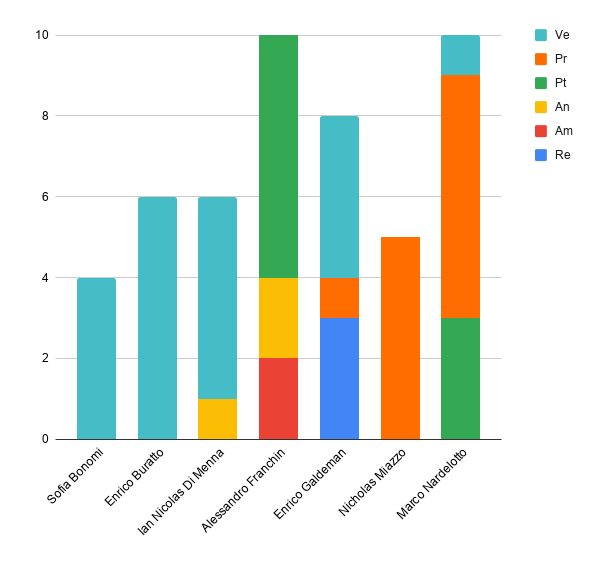
\includegraphics[width=12cm]{img/ore-4-incr.png}
    \caption{Istogramma della distribuzione oraria del quarto incremento}
    \label{fig:ore-componente-progettazione}
  \end{figure}

  \subsubsection{Prospetto economico}
  In questo periodo, la suddivisione oraria e i costi per ruolo è la seguente:

  \begin{table}[H]
    \centering
    \begin{tabular}{lcc}
      \rowcolor{lightgray}
      \textbf{Ruolo}  & \textbf{Ore previste} & \textbf{Costo}    \\
Responsabile    & 3                     & € 90,00           \\
Amministratore  & 2                     & € 40,00           \\
Analista        & 3                     & € 75,00           \\
Progettista     & 9                     & € 198,00          \\
Programmatore   & 12                    & € 180,00          \\
Verificatore    & 20                    & € 300,00          \\
\textbf{Totale} & \textbf{49}           & \textbf{€ 883,00}
    \end{tabular}
    \caption{Prospetto economico del quarto incremento}
  \end{table}


  Per facilitare la lettura della suddivisione oraria per ruolo, i dati vengono rappresentati graficamente mediante il seguente areogramma:
  \begin{figure}[H]
    \centering
    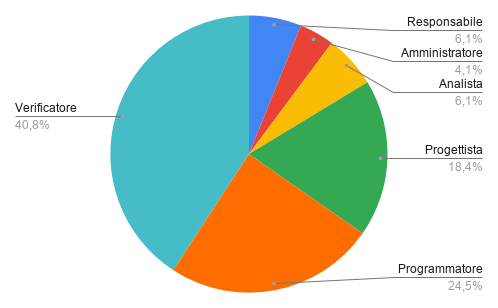
\includegraphics[width=12cm]{img/ruoli-4-incr.png}
    \caption{Areogramma della suddivisione dei ruoli del quarto incremento}
    \label{fig:ore-ruolo-progettazione}
  \end{figure}



\end{document}
